\documentclass[../main.tex]{subfiles}
\begin{document}
    Исследование из области солнечной энергетики [1]. На рис 1 показана схема установки для исследования фотоэлектрических характеристик.
    \begin{figure}[H]
    	\centering
    	    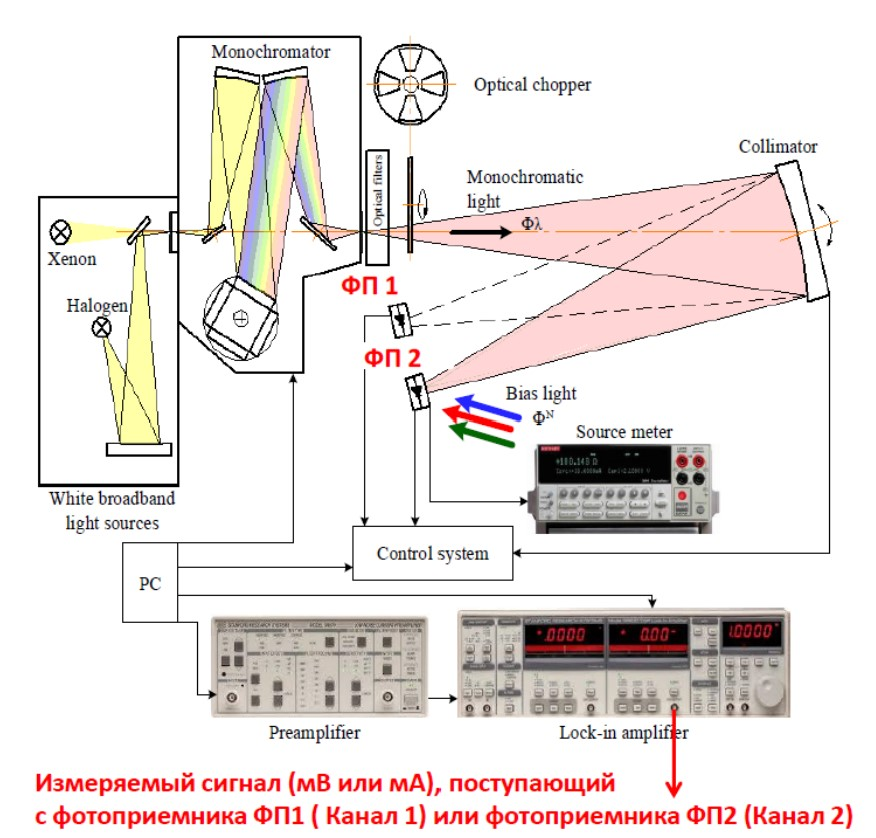
\includegraphics{figures/task.jpg}
    	\caption{Схема установки для исследования фотоэлектрических характеристик.}
    	\label{w_pert}
    \end{figure}
    
    Калибровка датчика ФП1 производится по эталону ФП2. Зависимость между квантовыми эффективностями датчиков предполагается одинаковой для каждой пары измерений
    \begin{equation}
        QE_{ФП2} = \frac{I_{ФП2}}{I_{ФП1}}*QE_{ФП1} 
        \label{T}
    \end{equation}
    QE - квантове эффективности эталонного и исследуемого датчиков, I - измеренные токи.
    
    \textbf{Исходные данные.}
    Имеется 2 выборки данных с интервальной неопределенностью. Одна из них относится к эталонному датчику ФП2, другая - к исследуемому датчику ФП1.
    
    \textbf{Задача.}
    Треубется определить коэффициент калибровки
    \begin{equation}
        R_{21} = \frac{I_{2}}{I_{1}}
        \label{T}
    \end{equation}
    при помощи линейной регрессии на множестве интервальных данных и коэффициента Жаккара.
\end{document}